%      File: VTthesis_template.tex
%     Created: Thu Mar 24 11:00 AM 2016 EDT
%     Last Change: Thursday, December 19, 2019
%     Author: Alan M. Lattimer, VT
%	  With modifications by Carrie Cross, Robert Browder, and LianTze Lim. 
%     modifications by Ziling Wu, PhD, Electrical and Computer Engineering department, VT, 2016-2020
% This template is designed to operate with XeLaTeX.
%
% All elements in the Title, Abstract, and Keywords MUST be formatted as text and NOT as math.
%
%Further instructions for using this template are embedded in the document. Additionally, there are comments at the end of the file that give suggestions on writing your thesis.  
%
%In addition to the standard formatting options, the following options are defined for the VTthesis class: proposal, prelim, doublespace, draft. 

\documentclass[doublespace,nopageskip]{VTthesis} % nopageskip - Removes arbitrary blank pages.

% Using the following header instead will create a draft copy of your thesis
%\documentclass[doublespace,draft]{VTthesis}

% The lipsum package is just included to put dummy text in the document in order to demonstrate page headers and table of contents behavior. You should remove it once you begin writing your actual thesis or dissertation.
\usepackage{lipsum}

% Title of your thesis
\title{Title of your thesis}

% You should include 3-5 keywords, separated by commas
\keywords{Some Keywords, Subject matter, etc.}

% Your name, including middle initial(s)
\author{Your Name}

% Change this to your program, e.g. Physics, Civil Engineering, etc.
\program{Your Department} 

% Change this to your degree, e.g. Master of Science, Master of Art, etc.
\degree{Doctor of Philosophy} 

% This should be your defense date:
\submitdate{December 4, 2020} 

% Committee members. Only have five readers and one chair available.
% Only use the ones you need and don't include the ones you don't need.
% You can also declare a Co-advisor. If you do, the principal and co-advisors
% will be listed as co-advisors on the title page.  Per the VT ETD standards, 
% you should not include titles or educational qualifications such as PhD or Dr.
% You should, however, include middle initials if possible.
\principaladvisor{Your Advisor}
%\coadvisor{Vicente Esparza}
\firstreader{First Committee}
\secondreader{Second Committee}
\thirdreader{Third Committee}
\fourthreader{Last Committee}

% The dedication and acknowledgement pages are optional. Comment them out to remove them.
\dedication{Dedicated to Virginia Tech.}
\acknowledge{\lipsum [1]}
 

% The abstract is required.
\abstract{Give a brief description of your thesis here.}
\abstract{\lipsum [1]}

% The general audience abstract is required. There are currently no word limits.
\abstractgenaud{You are also required as of Spring 2016 to include a general audience abstract. This should be geared towards individuals outside of your field that may be reading seeking information about your work. You should avoid language that is particular to your field and clearly define any terms that may have special meaning in your discipline. }

\begin{document}
% The following lines set up the front matter of your thesis or dissertation and are required to ensure proper formatting per the VT ETD standards. 
  \frontmatter
  \maketitle
  \tableofcontents

% The list of figures and tables are now optional per the official ETD standards.  Unless you have a very good reason for removing them, you should leave these lists in the document. Comment them out to remove them.
	\listoffigures
	\listoftables
	% sample text for abbreviations:
\nomenclature{NLP}{Natural Language Processing}
 
\nomenclature{$\sigma$}{The total mass of angels per unit area} 
    \printnomenclature %Creates a list of abbreviations. Comment out to remove it. 

% The following sets up the document for the main part of the thesis or dissertation. Do not comment out or remove this line.
	\mainmatter

	%now go ahead and start writing your thesis
	\chapter{Introduction} \label{ch:introduction}

\lipsum [1-2]
	\chapter{How to input figures}\label{ch:ch2}

Here shows to insert figures and cite figures in the main text.

\begin{figure}[h!]
\centering
\includegraphics[width = 0.85\linewidth]{./figs/ch2/lena.bmp}
\caption{Picture of Lena}
\label{fig:2-fig1}
\end{figure}
Picture of lena is shown in Fig. \ref{fig:2-fig1}.

	\chapter{How to input tables}\label{ch:ch3}

Here shows how we could input the table.

\begin{table}[h!]
\caption{Registered pore morphology variables}
\centering
\begin{tabular}{|m{2cm}|m{2cm}|m{2cm}|m{2cm}|m{2cm}|m{2cm}|m{2cm}|} 
\hline
metric 1 & metric 2 & metric 3& metric 4 & metric 5 & metric 6 & metric 7\\
\hline
a & b&	c&d&e&f&g\\
\hline
\end{tabular}
\label{tb:3-1}
\end{table}

You could also cite the table~\ref{tb:3-1} in this way.
    \chapter{How to input references} \label{ch:ch4}

In this chapter, I will discuss how I arrange the references that I feel make life much easier. You could have other ways if you prefer. 

I will take this reference as an example. 

\textit{Wu, Ziling, Tekin Bicer, Zhengchun Liu, Vincent De Andrade, Yunhui Zhu, and Ian T. Foster. "Deep Learning-based Low-dose Tomography Reconstruction with Hybrid-dose Measurements." arXiv preprint arXiv:2009.13589 (2020).}

If you use 'google scholar' search this article, here is what coming out from this search.

\begin{figure}[h!]
\centering

\includegraphics[width = 0.85\linewidth]{./figs/ch4/reference.PNG}
\caption{Google scholar search results}
\label{fig:4-fig1}
\end{figure}

After you click the symbol circled out in red shown in Fig.~\ref{fig:4-fig2}, multiple cite options will come out. You could click the BibTex in green box and you could get the format to cite this article in a new page. You could copy all text in the new page to the 'ref.bib' file in the reference folder and it is ready to cite~\cite{wu2020deep} now. 

\begin{figure}[h!]
\centering
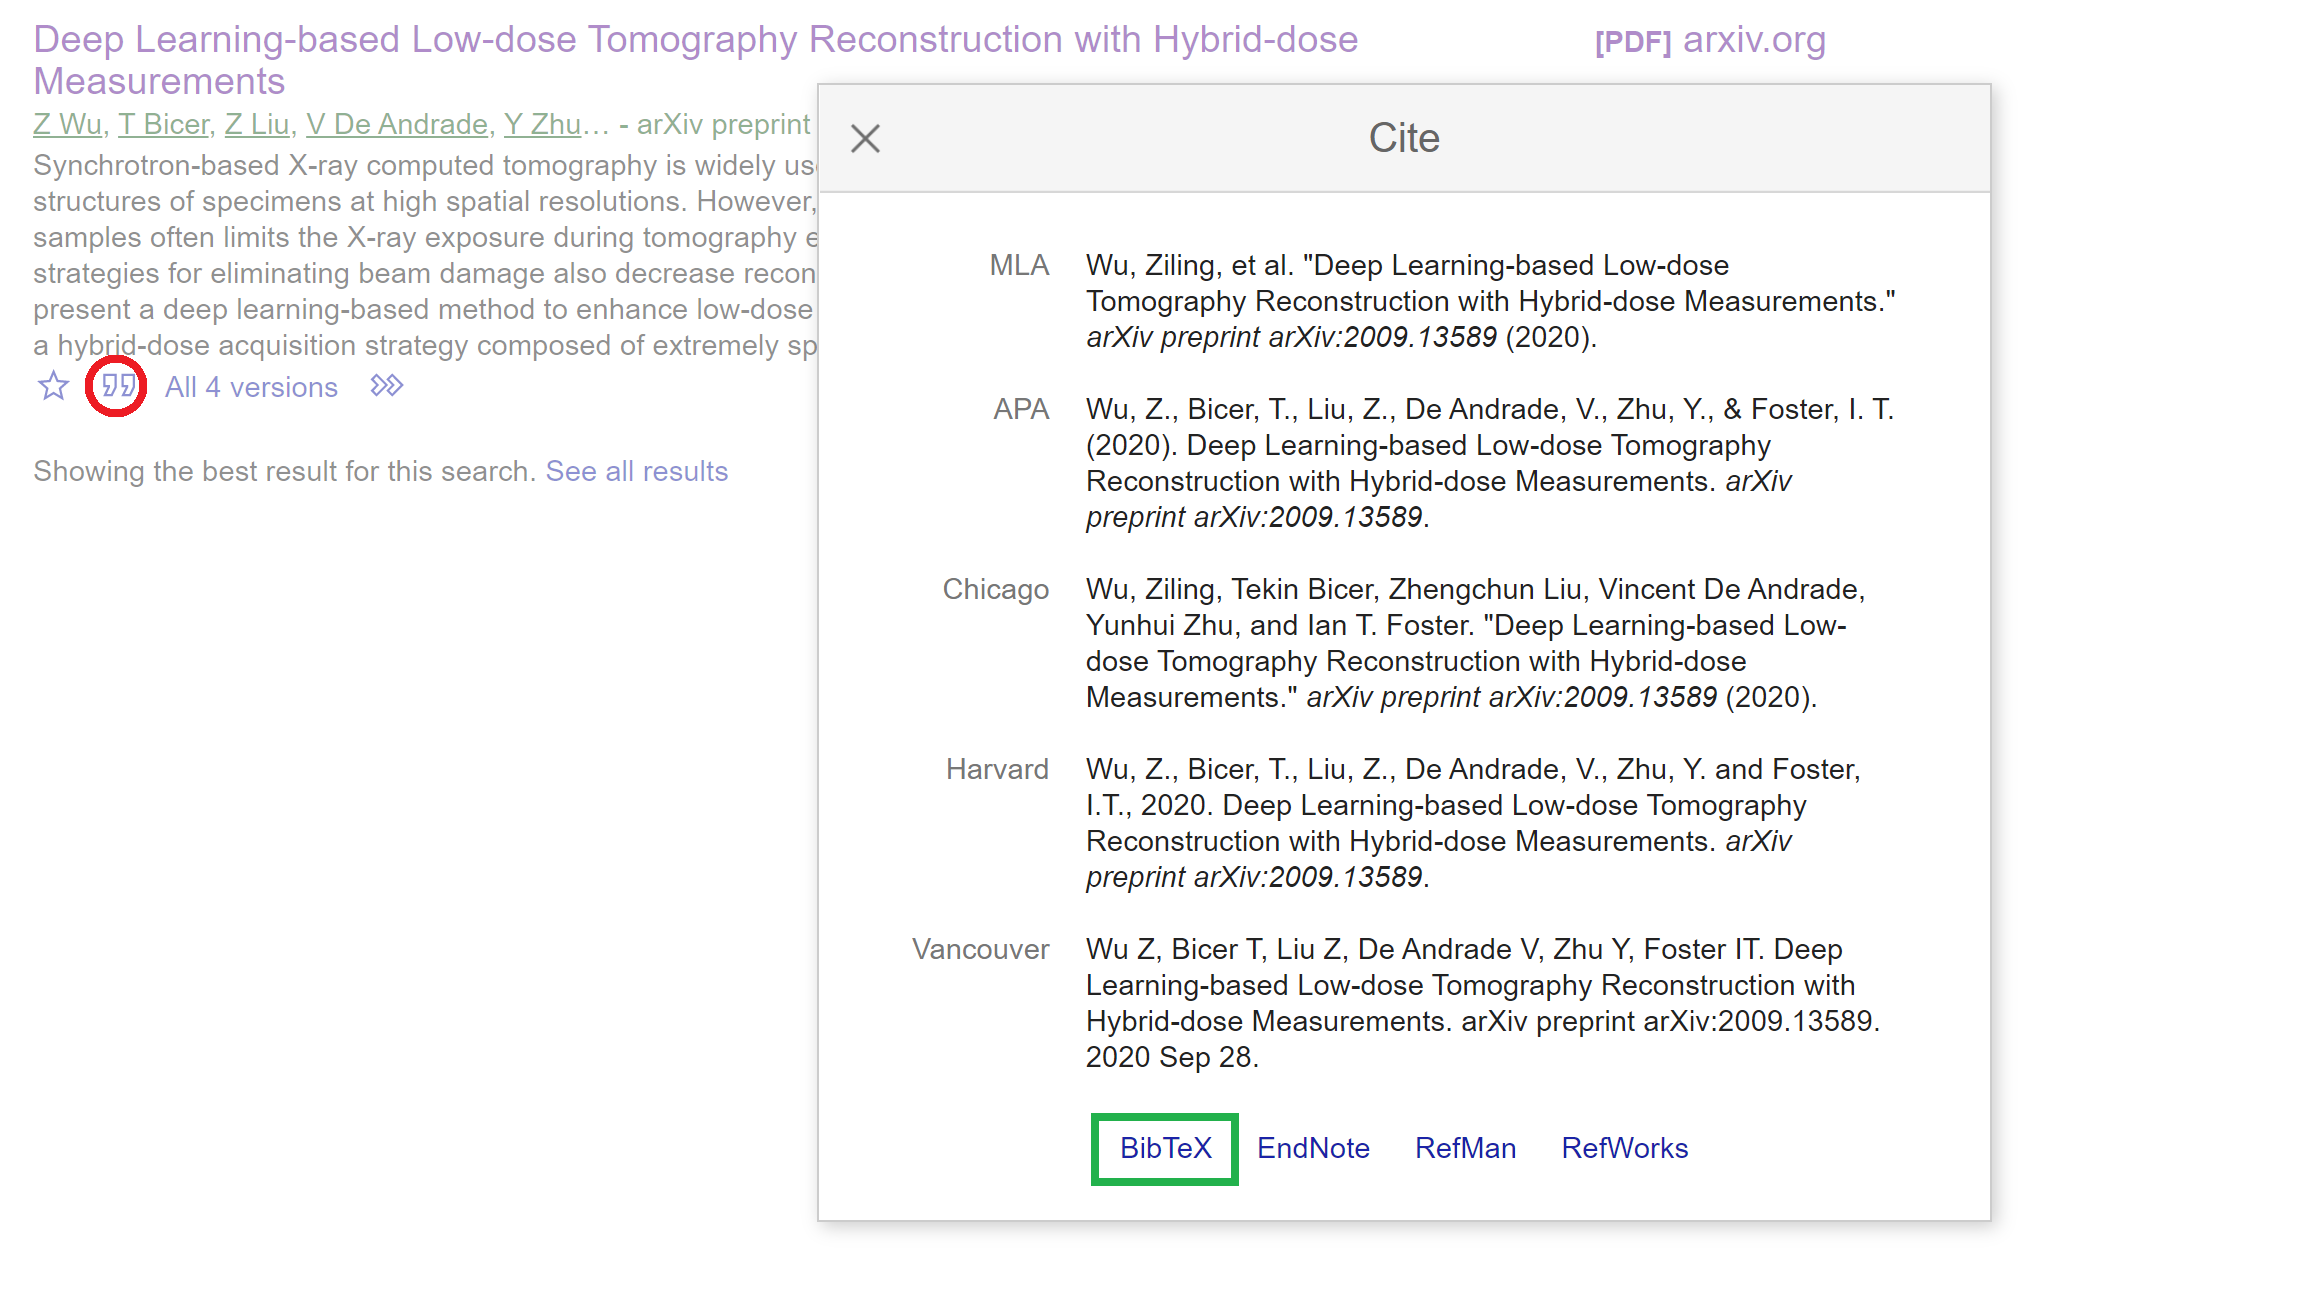
\includegraphics[width = 0.85\linewidth]{./figs/ch4/bibTex.png}
\caption{Google scholar search results}
\label{fig:4-fig2}
\end{figure}


	

	% This is the standard bibtex file. Do not include the .bib extension in <bib_file_name>.
	% Uncomment the following lines to include your bibliography: 
	%\bibliography{<bib_file_name>}
	%\bibliographystyle{plainnat}   

	% This formats the chapter name to appendix to properly define the headers:
	\appendix

	% Add your appendices here. You must leave the appendices enclosed in the appendices environment in order for the table of contents to be correct.
	
\begin{appendices}
\chapter{Appendices I} \label{app:appendix_one}
\section{A1} \label{ase:app_one_sect_1}
\section{A2} \label{ase:app_one_sect_2}
% \chapter{Second Appendix} \label{app:appendix_two}
\end{appendices}
    \bibliography{./reference/ref}
    \bibliographystyle{ieeetr}  
\end{document}



%****************************************************************************
% Below are some general suggestions for writing your dissertation:
%
% 1. Label everything with a meaningful prefix so that you
%    can refer back to sections, tables, figures, equations, etc.
%    Usage \label{<prefix>:<label_name>} where some suggested
%    prefixes are:
%			ch: Chapter
%     		se: Section
%     		ss: Subsection
%     		sss: Sub-subsection
%			app: Appendix
%     		ase: Appendix section
%     		tab: Tables
%     		fig: Figures
%     		sfig: Sub-figures
%     		eq: Equations
%
% 2. The VTthesis class provides for natbib citations. You should upload
%	 one or more *.bib bibtex files. Suppose you have two bib files: some_refs.bib and 
%    other_refs.bib.  Then your bibliography line to include them
%    will be:
%      \bibliography{some_refs, other_refs}
%    where multiple files are separated by commas. In the body of 
%    your work, you can cite your references using natbib citations.
%    Examples:
%      Citation                     Output
%      -------------------------------------------------------
%      \cite{doe_title_2016}        [18]
%      \citet{doe_title_2016}       Doe et al. [18]
%      \citet*{doe_title_2016}      Doe, Jones, and Smith [18]
%
%    For a complete list of options, see
%      https://www.ctan.org/pkg/natbib?lang=en
%
% 3. Here is a sample table. Notice that the caption is centered at the top. Also
%    notice that we use booktabs formatting. You should not use vertical lines
%    in your tables.
% 
%				\begin{table}[htb]
%					\centering
%					\caption{Approximate computation times in hh:mm:ss for full order 						versus reduced order models.}
%					\begin{tabular}{ccc}
%						\toprule
%						& \multicolumn{2}{c}{Computation Time}\\
%						\cmidrule(r){2-3}
%						$\overline{U}_{in}$ m/s & Full Model & ROM \\
%						\midrule
%						0.90 & 2:00:00 & 2:08:00\\
%						0.88 & 2:00:00 & 0:00:03\\
%						0.92 & 2:00:00 & 0:00:03\\
%						\midrule
%						Total & 6:00:00 & 2:08:06\\
%						\bottomrule
%					\end{tabular}
%					\label{tab:time_rom}
%				\end{table}
% 
% 4. Below are some sample figures. Notice the caption is centered below the
%    figure.
%    a. Single centered figure:
%					\begin{figure}[htb]
%						\centering
%						\includegraphics[scale=0.5]{my_figure.eps}
%						\caption{Average outlet velocity magnitude given an average  
%				        input velocity magnitude of 0.88 m/s.} 
%						\label{fig:output_rom}
%					\end{figure}
%    b. Two by two grid of figures with subcaptions
%					\begin{figure}[htb]
%						\centering
%						\begin{subfigure}[h]{0.45\textwidth}
%							\centering
%							\includegraphics[scale=0.4]{figure_1_1.eps}
%							\caption{Subcaption number one}
%							\label{sfig:first_subfig}
%						\end{subfigure}
%						\begin{subfigure}[h]{0.45\textwidth}
%							\centering
%							\includegraphics[scale=0.4]{figure_1_2.png}
%							\caption{Subcaption number two}
%							\label{sfig:second_subfig}
%						\end{subfigure}
%
%						\begin{subfigure}[h]{0.45\textwidth}
%							\centering
%							\includegraphics[scale=0.4]{figure_2_1.pdf}
%							\caption{Subcaption number three}
%							\label{sfig:third_subfig}
%						\end{subfigure}
%						\begin{subfigure}[h]{0.45\textwidth}
%							\centering
%							\includegraphics[scale=0.4]{figure_2_2.eps}
%							\caption{Subcaption number four}
%							\label{sfig:fourth_subfig}
%						\end{subfigure}
%						\caption{Here is my main caption describing the relationship between the 4 subimages}
%						\label{fig:main_figure}
%					\end{figure}
%
%----------------------------------------------------------------------------
%
% The following is a list of definitions and packages provided by VTthesis:
%
% A. The following packages are provided by the VTthesis class:
%      amsmath, amsthm, amssymb, enumerate, natbib, hyperref, graphicx, 
%      tikz (with shapes and arrows libraries), caption, subcaption,
%      listings, verbatim
%
% B. The following theorem environments are defined by VTthesis:
%      theorem, proposition, lemma, corollary, conjecture
% 
% C. The following definition environments are defined by VTthesis:
%      definition, example, remark, algorithm
%
%----------------------------------------------------------------------------
%
%  I hope this template file and the VTthesis class will keep you from having 
%  to worry about the formatting and allow you to focus on the actual writing.
%  Good luck, and happy writing.
%    Alan Lattimer, VT, 2016
%
%****************************************************************************





